\chapter{Event Reconstruction}
\label{sec:event:reco}

The particles produced in the \gls{pp} collisions in the center of the \gls{atlas} detector, interact with the detector material as discussed in Chapter \ref{chap:cern}. As a result of these interactions, electrical currents are recorded. \textit{Event reconstruction} is the process of recombining these digital signals and interpreting them as tracks and energy deposits in the calorimeters. A further step consists in analyzing the characteristics of the candidate tracks and calorimeter clusters and identify them as signs of the passage of specific particles.
This chapter describes the reconstruction and identification of the objects used in the analyses discussed in this thesis: tracks and vertices, electrons, muons, hadronic jets and missing transverse momentum. 


\subsection{Tracks and Primary Vertices}
\label{sec:reco:tracks}

In \gls{atlas} the identification of tracks from charged particles relies on the information collected by the \gls{id}. The tracking information is crucial to the reconstruction and identification of many types of particles, including electrons, muons, and the jest originating from the hadronization of a b-quark. The precision on the position measurement of the track depends on the granularity of the different subsystems of the \gls{id} and, since the \gls{id} is surrounded by a solenoidal magnetic field, the charged particles follow an helical trajectory. After the point of closest approach (perigee) to a given reference is defined, the trajectory of the track can be described by five parameters: 
\begin{equation}
\theta, \; \phi, \; q/p \; d_0, \; z_0 \;,
\end{equation}
\noindent where $\theta$ and $\phi$ are the azimuthal and polar angle, $q/p$ is the ratio of the charge of the track to the track momentum, and $d_0$ and $z_0$ are the distance to the point of closest approach in the transverse plane and along the $z$-axis. 

Primary tracks, originating from the hard-scattering vertex, are reconstructed with an inside-out approach \cite{Cornelissen:1020106}: the seed of the reconstruction are three hits in the silicon detector, and then compatible hits in the outer layers of the \gls{id} are added with a Kalman Filter \cite{citeulike:347166,Fruhwirth:1987fm}. The \gls{trt} segments that are not associated with primary tracks are used as starting point to reconstruct tracks from long-lived particles or from material interaction, with a back-tracking that extrapolates the \gls{trt} information to the pixel hits. 

Random groups of hits can be wrongly reconstructed as belonging to the helical trajectory of a track (\textit{fake tracks}). The amount of fake tracks increases with the increase of pile-up, and can be reduced by tightening the selection criteria of the track, at the expense of reconstruction efficiency. Three different selection criteria are used for the data collected in 2015 and 2016 (Loose, Loose-Primary and Tight-Primary), that differ in the requirements on the hits and holes (elements where a hit was expected but was not registered) in the different \gls{id} layers. The \textit{track reconstruction efficiency} is measured in \gls{mc} simulations as the ratio of the reconstructed tracks matched to a generated charged particle over the total number of generated charged particles. The reconstruction efficiency as a function of the track $\eta$ and \pt is shown in Fig. \ref{fig:obj:tracks} for Loose and Tight-Primary tracks.
 
\begin{figure}[ht]
\centering
\subfigure[]{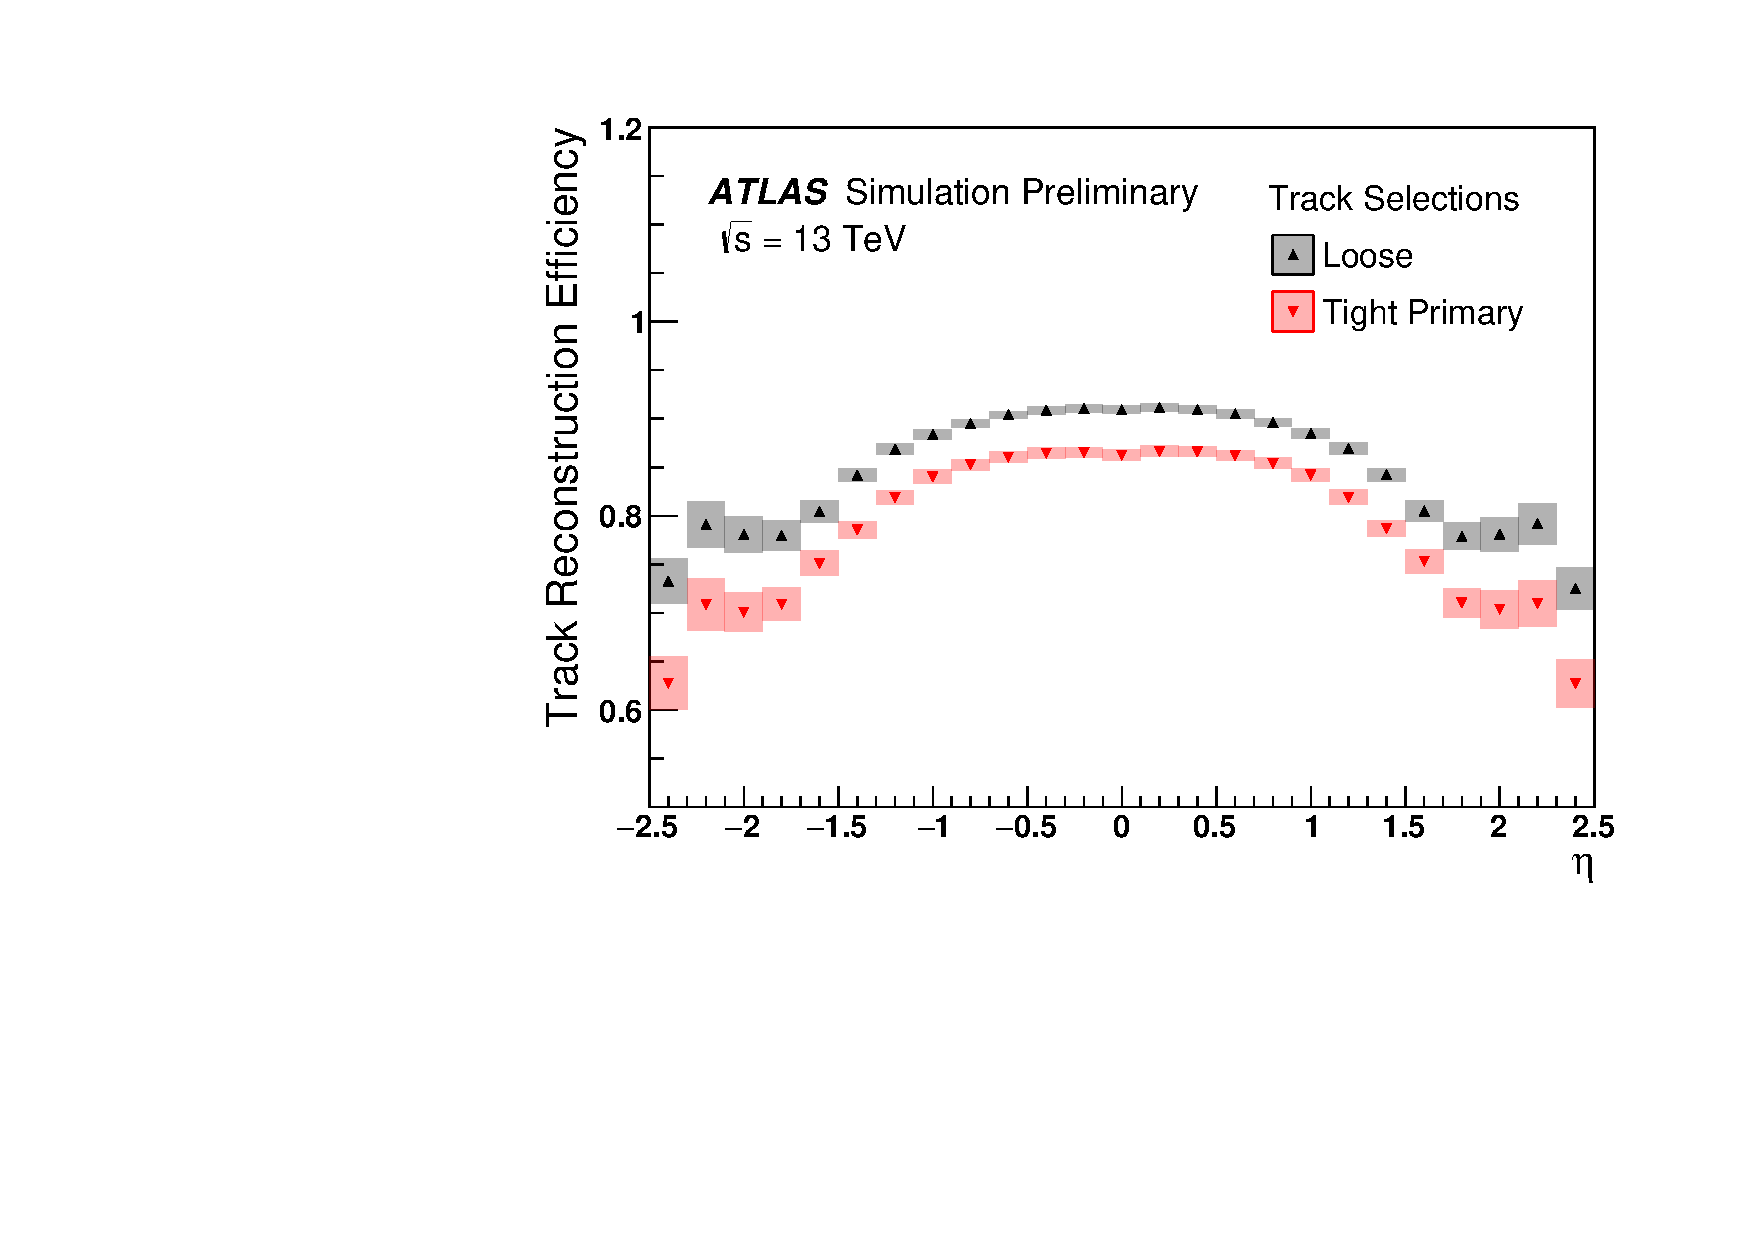
\includegraphics[width=0.48\textwidth]{figures/objects/track1}}
\subfigure[]{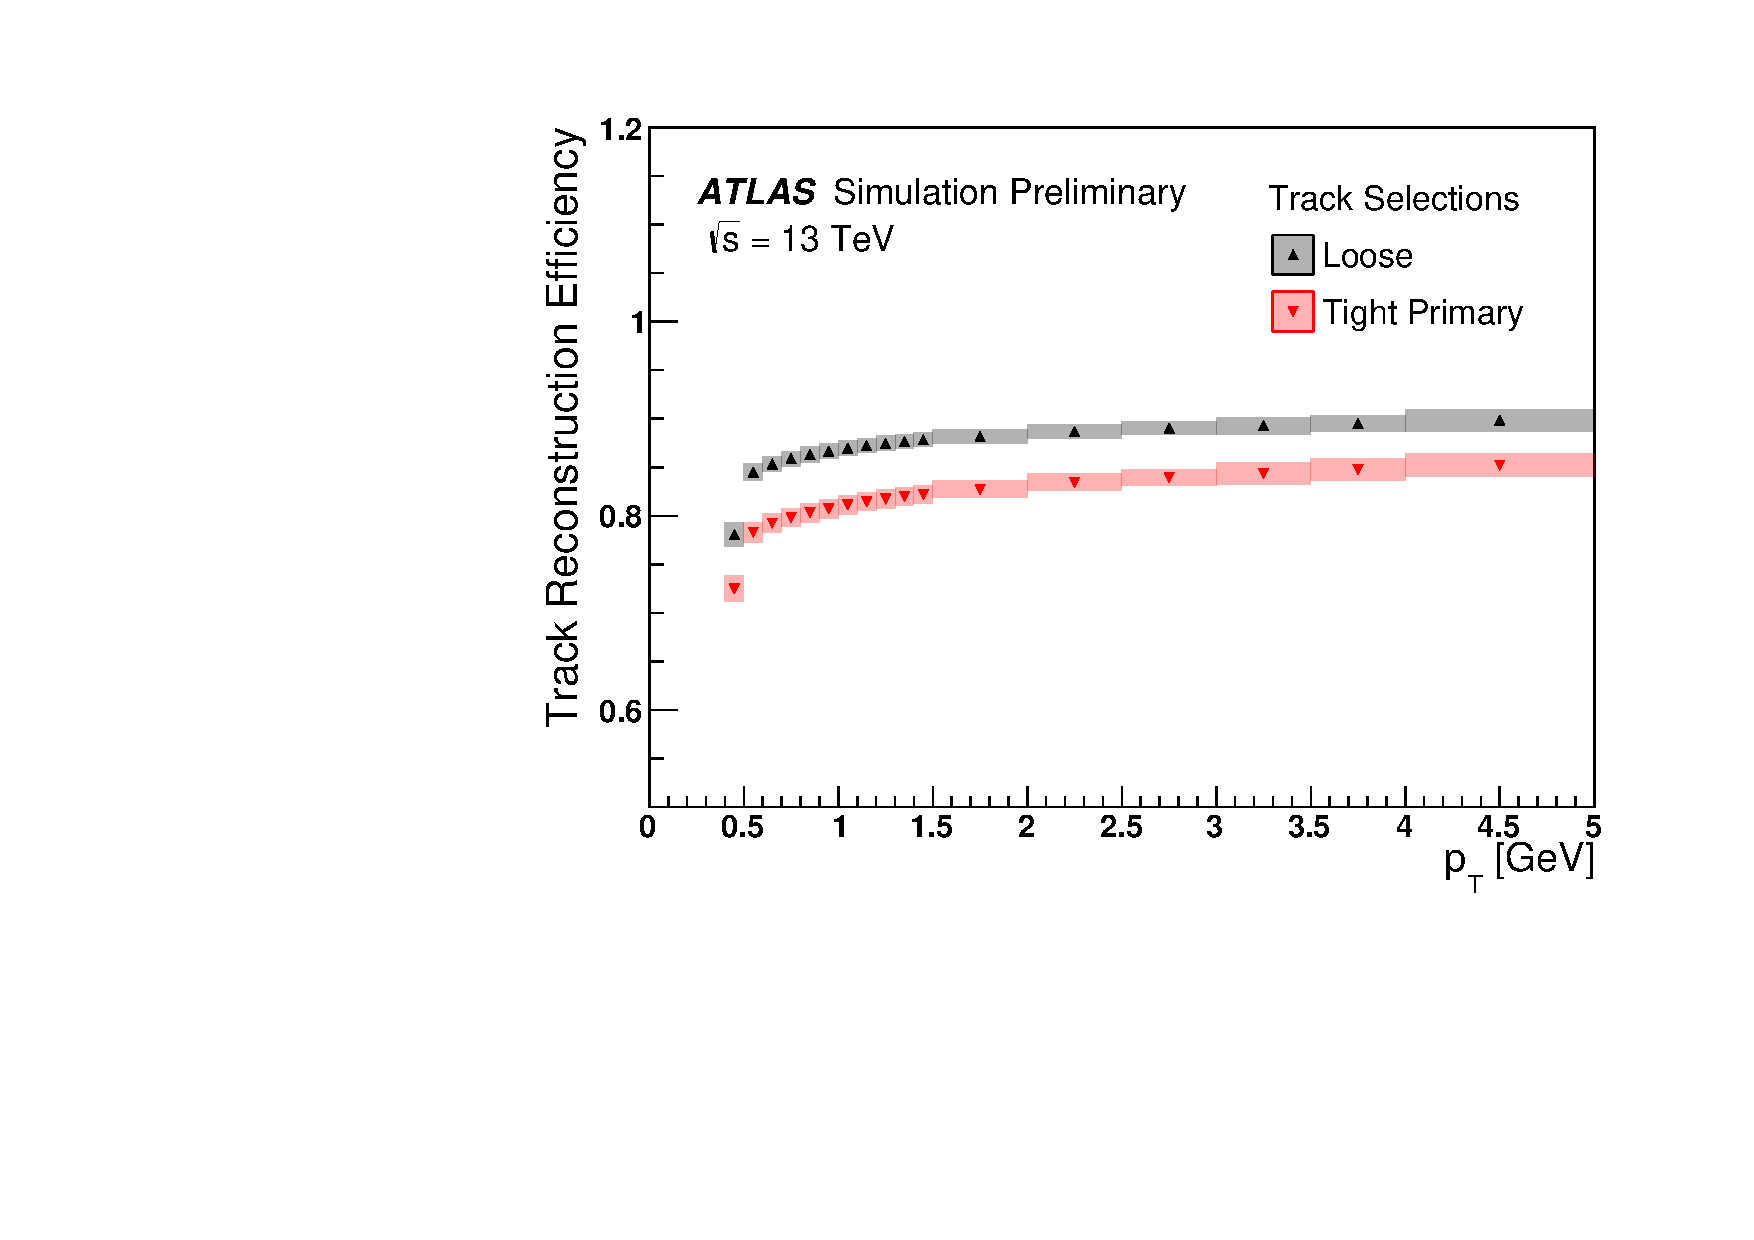
\includegraphics[width=0.48\textwidth]{figures/objects/track2}}
\caption{Track reconstruction efficiency, evaluated by using minimum bias simulated events, as a function of truth $\eta$ (a) and \pt (b) for Loose and Tight Primary track selections.The bands indicate the total sstematic uncertainty. Figure from Ref. \cite{ATL-PHYS-PUB-2015-051}.}
\label{fig:obj:tracks}
\end{figure}

Tracks are the starting point for the identification of vertices. \glspl{pv} are reconstructed through a vertex fitting algorithm. Once all the \glspl{pv} are reconstructed, the one with the highest sum of the squared transverse momenta of its associated tracks ($\sum_i^{N-tracks}p_{T,i}^2$) is identified as the hard scattering vertex, and $d_0$ and $z_0$ are recomputed with respect to its coordinates. The other vertices are named pile-up vertices, and their number is correlated  to the number of interactions per bunch crossing.


\subsection{Hadronic Jets}

\subsubsection{Jets from B-hadrons}


\subsection{Electrons}

\subsection{Muons}

\subsection{Missing Transverse Momentum}

Particles that interact only weakly with the detector, such as neutrinos or BSM particles like neutralinos, are not reconstructed directly. 
Their presence is instead inferred by measuring the total momentum imbalance in the event. 